\subsection{Logiche TTL e scheda di visualizzazione}
Le porte logiche a tecnologia TTL funzionano utilizzando come 1 logico il valore di tensione +\SI{5}{\volt} mentre come 0 logico \SI{0}{\volt}.
Pertanto l'alimentazione che porteremo alla breadboard non sarà più $\pm$\SI{15}{\V} e GND, ma solo $+$\SI{5}{\V} e GND.
Ricordiamo che l'alimentazione deve essere stabilizzata e disaccoppiata con i condensatori come nel caso analogico in quanto nei momenti di commutazione delle porte abbiamo grandi variazioni di tensione in piccoli tempi (idealmente la variazione da stato 1 a 0 è istantanea).
È dunque essenziale avere una riserva di cariche utilizzabili dal circuito nel momento in cui si hanno commutazioni.

RESITENZE DI PULL-UP E PULL-DOWN

Per controllare il funzionamento dei nostri circuiti utilizzeremo una schedina di visualizzazione a led fornitaci già assemblata.
Essa permette di visualizzare lo stato "alto" o "basso" delle linee da monitorare tramite 8 led (4 rossi e 4 verdi).
Tali schede contengono un integrato buffer 74LS244 nella logica TTL che fornisce in uscita una corrente di \SI{-15}{\milli\ampere} per il livello alto e di \SI{24}{\milli\ampere} per il livello basso.
% NON HO IDEA SE LA PARTE DEL 74LS244 SIA CORRETTA O MENO (xD)

\subsubsection{Porta NAND}

\begin{wrapfigure}[5]{r}{0.4\textwidth}
\centering
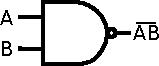
\includegraphics[width=.15\textwidth]{../E09/latex/NAND.pdf}
\caption{Simbolo circuitale convenzionalmente utilizzato per porte NAND.}
\label{cir9:nand}
\end{wrapfigure}

Abbiamo verificato il funzionamento di una porta NAND utilizzando, come già detto, una scheda di visualizzazione a LED.
È stata verificata la seguente tavola di verità.\\

\vspace{-5mm}
\begin{table}[htpc]
\begin{minipage}{0.6\textwidth}
\centering
{\renewcommand{\arraystretch}{1.2}%
\begin{tabular}{|c|c|c|}
\hline
A & B & $\overline{AB}$ \\
\hline
0 & 0 & 1\\
\hline
0 & 1 & 1\\
\hline
1 & 0 & 1\\
\hline
1 & 1 & 0\\
\hline
\end{tabular}}
\label{tab9:NAND}
\end{minipage}
\end{table}
\vspace{-4mm}

\subsubsection{Porta NOT}


\begin{wrapfigure}[10]{r}{0.4\textwidth}
\centering
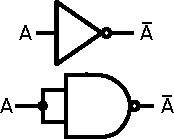
\includegraphics[width=.16\textwidth]{../E09/latex/NOT.pdf}
\caption{Implementazione e simbolo circuitale per porte NOT.}
\label{cir9:not}
\end{wrapfigure}

Non avendo a disposizione una porta NOT, abbiamo utilizzato una porta NAND cortocircuitando i due ingressi tra loro.
Così facendo otteniamo un'implementazione di una porta NOT.

Ne abbiamo ininzialmente verificato il funzionamento collengandola alla scheda di visualizzazione led e fornendo un'onda quadra in ingresso ($V_{pp}=\SI{5}{\volt}$, $V_{off}=+\SI{2.5}{\volt}$, $\nu=\SI{2}{\hertz}$).
Una volta eseguito questo test preliminare, abbiamo collegato ingresso ed uscita all'oscilloscopio e ne abbiamo analizzato la risposta per diverse tensioni costanti in ingresso.
I dati ottenuti sono riportati in Tabella (\ref{tab9:risposta2}).
Come vediamo, tra \SI{1}{\volt} e \SI{1.5}{\volt} la tensione varia in modo molto rapido.

%\begin{table}[htpc]
%\centering
%\begin{tabular}{|l|l|||l|l|||l|l|||l|l|}
%\hline
%$V_{in}$ [\si{\volt}] & $V_{out}$ [\si{\volt}] & $V_{in}$ [\si{\volt}]& $V_{out}$ [\si{\volt}] & $V_{in}$ [\si{\volt}]& $V_{out}$ [\si{\volt}] & $V_{in}$ [\si{\volt}]& $V_{out}$ [\si{\volt}]\\
%\hline
%0 & 4.30 & 2.5 & 0.10 & 5  & 0.10 & 2.5 & 0.10\\
%\hline
%0.5 & 4.05 & 3 & 0.10 & 4.5 & 0.10 & 2 &0.10\\
%\hline
%1 & 3.01 & 3.5 & 0.10 & 4 & 0.10 & 1.5 & 0.10\\
%\hline
%1.5 & 0.10 & 4 & 0.10 & 3.5 & 0.10 & 1 & 3.00\\
%\hline
%2 & 0.10 & 4.5 & 0.10 & 3.0 &0.10 & 0.5 & 4.05\\
%\hline
%\end{tabular}
%\label{tab9:risposta}
%\end{table}

\begin{table}[htpc]
\centering
{\renewcommand{\arraystretch}{1.1}%
\begin{tabular}{l|c|c|c|c|c|c|c|c|c|c|c}
$V_{in}$ [\si{\volt}] & 0.0 & 0.5 & 1.0 & 1.5 & 2.0 & 2.5 & 3.0 & 3.5 & 4.0 & 4.5 & 5.0 \\
\hline
$V_{out}$ [\si{\volt}] & 4.30 & 4.05 & 3.01 & 0.10 & 0.10 & 0.10 & 0.10 & 0.10 & 0.10 & 0.10 & 0.10 \\
\end{tabular}}
\caption{I valori sono stati ricavati variando la tensione in entrata di \SI{.5}{\V}.}
\label{tab9:risposta2}
\end{table}

Siamo dunque interessati a capire meglio la risposta della porta in funzione della tensione in ingresso.
Per fare ciò utilizziamo la modalità XY dell'oscilloscopio.

Abbiamo dunque fornito un'onda sinusoidale all'ingresso di frequenza \SI{100}{\kilo\hertz}, $V_{pp}=\SI{5}{\volt}$ e $V_{off}=+\SI{2.5}{\volt}$.
Come vediamo dal grafico sotto riportato, sebbene stiamo lavorando con segnali digitali (1 o 0) le tensioni in gioco sono manifestamente analogiche.
Avremo dunque tutta la serie di problemi già affrontati nella parte analogica del corso.
Vediamo infatti che la tensione in uscita non è una funzione a gradino.
Inoltre, per evitare che rumori molesti disturbino il segnale in uscita, avremo bisogno di una sorta di isteresi.
Non esisterà dunque un valore ben definito di V alta e V bassa, ma delle bande di lavoro standard per la classe di circuiteria scelta (nel nostro caso TTL), riportate solitamente nel data-sheet.
Lo standard TTL è riportato in Figura \ref{fig9:TTL}

\begin{figure}[htpc]
\centering
	\begin{subfigure}[hc]{0.49\textwidth}
		\centering
		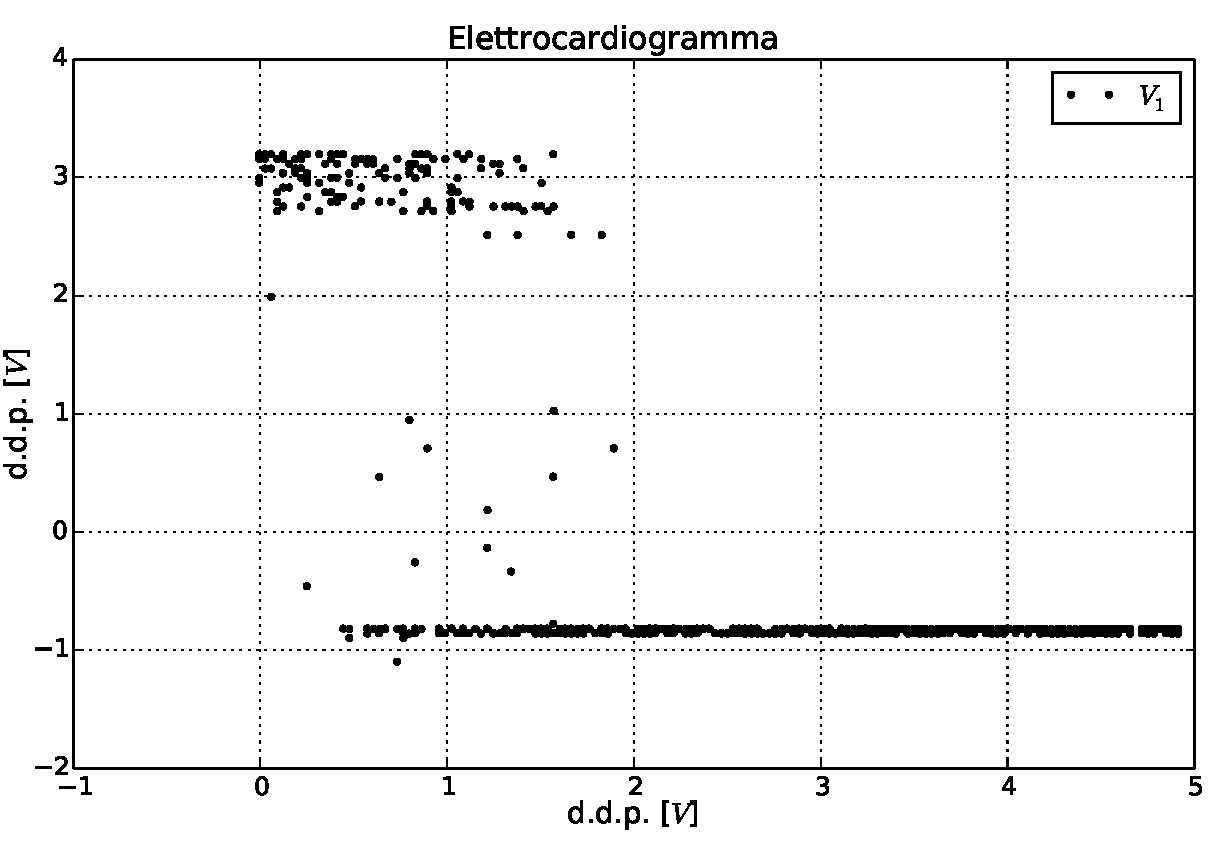
\includegraphics[width=.95\textwidth]{../E09/latex/XYschifo.pdf}
                \caption{XY.}
                \label{fig9:XY}
        \end{subfigure}%
	\quad
        \begin{subfigure}[hc]{0.49\textwidth}
		\centering
		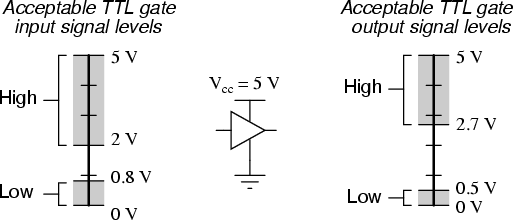
\includegraphics[width=.95\textwidth]{../E09/latex/TTL.png}
                \caption{Livelli standard di input e output per la logica TTL.}
                \label{fig9:TTL}
        \end{subfigure}
\caption{}
\end{figure}
\vspace{-5mm}

\subsubsection{Circuito di GATE con porta AND}
Per realizzare il circuito GATE è sufficiente utilizzare una porta AND con un segnale di controllo ad un ingresso.
Per realizzare una porta AND possiamo utilizzare 2 NAND come proposto nella seguente figura.
Infatti, utilizzando la notazione convenzionale, $AB=\overline {\overline {AB}}$ che trivialmente è una NAND e una NOT in serie.
 
\begin{wrapfigure}[3]{r}{0.4\textwidth}
\centering
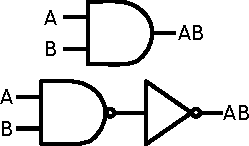
\includegraphics[width=.22\textwidth]{../E09/latex/AND.pdf}
\caption{Implementazione e simbolo circuitale per porte AND.}
\label{cir9:AND}
\end{wrapfigure}

La tavola di verità è la seguente (A=C=controllo, B=S=segnale):

%\vspace{-5mm}
\begin{table}[htpc]
\begin{minipage}{0.6\textwidth}
\centering
{\renewcommand{\arraystretch}{1.1}%
\begin{tabular}{|l|l|c|}
\hline
C & S & CS \\
\hline
0 & 0 & 0\\
\hline
0 & 1 & 0\\
\hline
1 & 0 & 0\\
\hline
1 & 1 & 1\\
\hline
\end{tabular}}
\label{tab9:AND}
\end{minipage}
\end{table}
%\vspace{-4mm}

Come vediamo dalla tabella, se il segnale di controllo è a 0 logico l'uscita sarà sempre 0 logico.
Se invece il controllo è a 1 logico, allora l'uscita sarà una copia del segnale in ingresso.
Per verificare empiricamente ciò, abbiamo collegato l'oscilloscopio all'uscita del circuito e fornito un'onda quadra ($V_{pp}=\SI{5}{\volt}$, $V_{off}=+\SI{2.5}{\volt}$, $\nu=\SI{2}{\hertz}$).
Abbiamo visto che quando il controllo era collegato a comune, l'uscita era praticamente nulla (\num{40} -- \SI{60}{\mV}).
Con il controllo a 0 logico, abbiamo osservato invece la stessa onda quadra posta in ingresso anche in uscita.

\subsubsection{Porta XOR}

Una porta XOR implementa la funzione matematica della somma diretta.
Avendo solo a disposizione porte NAND, dobbiamo cercare di implementare un circuito che svolga tale funzione.

\begin{wrapfigure}[8]{r}{0.4\textwidth}
\centering
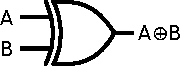
\includegraphics[width=.330\textwidth]{../E09/latex/XOR.pdf}
\caption{Implementazione e simbolo circuitale per porte XOR.}
\label{cir9:XOR}
\end{wrapfigure}

Riportiamo a seguire la tavola di verità per questa porta.
%In questo semplice caso non è necessario scomodare dalla tomba il povero Karnaugh.

%\vspace{-3mm}
\begin{table}[htpc]
\begin{minipage}{0.6\textwidth}
\centering
{\renewcommand{\arraystretch}{1.1}%
\begin{tabular}{|c|c|c|}
\hline
A & B & $A \oplus B$ \\
\hline
0 & 0 & 0\\
\hline
0 & 1 & 1\\
\hline
1 & 0 & 1\\
\hline
1 & 1 & 0\\
\hline
\end{tabular}}
\label{tab9:XOR}
\end{minipage}
\end{table}
%\vspace{-4mm}

Senza utilizzare le mappe di Karnaugh, è facile vedere che vale $A \oplus B=A\overline B + \overline A B$ e applicando il teorema di De Morgan si ottiene:  %, dove con A,B indichiamo l'1 logico, con $\overline A,\overline B$ lo 0 logico.

$$A \oplus B=A\overline B + \overline A B=\overline{\overline{A\overline B + \overline A B}}=\overline{\overline{A\overline B} \cdot \overline{\overline A B}}$$

Dunque, il circuito per realizzare una porta XOR usando porte NAND e NOT è riportato in Figura \ref{cir9:XOR}.

Come vediamo, la realizzazione da noi progettata prevede l'utilizza do 2 porte NOT e 3 NAND.
Ne abbiamo verificato il funzionamento con la scheda a LED.

\newpage

\subsubsection{Votazione con 3 Giurati e 1 Presidente}
Consideriamo un'assemblea composta da tre giurati e un presidente il cui compito è votare a favore o contro QUALCOSA, in cui il voto del presidente vale il doppio.
Il circuito che restituisce l'esito della votazione prevede di sommare i voti dei vari membri tenendo però in considerazione che il voto del presidente ha peso doppio.
Se la maggioranza dei voti ($\geq 50\%$) è positiva allora la votazione ha esito positivo, altrimenti ha esito negativo.

\begin{wraptable}[7]{c}{.4\textwidth}%[htpc]
%\begin{minipage}{0.6\textwidth}
\centering
{\renewcommand{\arraystretch}{1}%
\begin{tabular}{|c|c|c|c|c|}
\hline
\diaghead{\theadfont lololololo a} {CP}{AB}& 00 & 01 & 11 & 10\\
%\diaghead{}{CP}{AB}& 00 & 01 & 11 & 10\\
\hline
00 & 0 & 0 & 0 & 0 \\
\hline
01 & 0 & 1 & 1 & 1 \\
\hline
11 & 1 & 1 & 1 & 1 \\
\hline
10 & 0 & 0 & 1 & 0 \\
\hline
\end{tabular}}
\caption{}
\label{tab9:giurati}
%\end{minipage}
\end{wraptable}

Partiamo dunque dalla mappa di Karnaugh riportata in Tabella \ref{tab9:giurati}: minimizzando tale mappa otteniamo

$$Y=ABC+P(A+B+C)$$

Come fatto prima, avendo a disposizione solo porte NAND, trasformiamo tutto in prodotti.

%\begin{align}
%Y 	&= ABC+P(A+B+C)
%	= \overline{\overline{ABC+P(A+B+C)}} %\nonumber \\
%	= \overline{\overline{ABC} \cdot \overline {P(A+B+C)} }
%	= \overline{\overline{(AB)C} \cdot \overline {P(\overline{\overline{{A+B+C}} })}} \nonumber \\
%	&= \overline{\overline{(AB)C} \cdot \overline {P(\overline{{(\overline A \cdot \overline B) %\cdot \overline C} })}} %\nonumber
%\end{align}

\vspace{-1mm}
\begin{minipage}{0.6\textwidth}
\begin{align}
Y 	&= ABC+P(A+B+C)
	= \overline{\overline{ABC+P(A+B+C)}} \nonumber \\
	&= \overline{\overline{ABC} \cdot \overline {P(A+B+C)} }
	= \overline{\overline{(AB)C} \cdot \overline {P(\overline{\overline{{A+B+C}} })}} \nonumber \\
	&= \overline{\overline{(AB)C} \cdot \overline {P(\overline{{(\overline A \cdot \overline B) \cdot \overline C} })}} \nonumber
\end{align}
\end{minipage}
\vspace{3mm}

Ora è immediato costruire il circuito utilizzando porte NAND e NOT.
Lo schema è riportato in Figura \ref{cir9:giudici}.\\
Come per gli altri circuiti, ne è stato verificato utilizzando la schedina a LED. 

\begin{figure}[htpc]
\centering
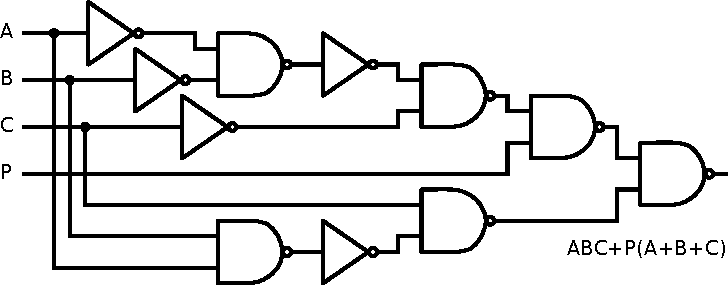
\includegraphics[width=.75\textwidth]{../E09/latex/giudici.pdf}
\caption{Circuito logico dedicato alla votazione di una assemblea collegiale composta da un presidente e tre giurati.}
\label{cir9:giudici}
\end{figure}

\subsubsection{Allarme per appartamento}

In quest'ultima parte dell'esperienza cercheremo di progettare e costruire un circuito di allarme.
%\sout{Immaginiamo di avere una villa piena di zoccole e di aver installato dei sensori.}
Immaginiamo di avere un mini-appartamento in cui sono presenti sensori d'apertura su porte e finestre e un sensore di movimento.
Vogliamo analizzarne i segnali per decidere se fare suonare l'allarme.

Chiamiamo P il sensore sulla porta (0=chiusa), F il sensore sulla finestra (0=chiusa), I il sensore ad infrarossi (0=no movimento) e infine C la chiave che permette di attivare l'allarme escludendo il sensore ad infrarossi (1=escludo infrarossi).

\begin{wraptable}[11]{c}{.4\textwidth}%[htpc]
%\begin{minipage}{0.6\textwidth}
\centering
{\renewcommand{\arraystretch}{1}%
\begin{tabular}{|c|c|c|c|c|}
\hline
\diaghead{\theadfont lololololo a} {IC}{PF}& 00& 01 & 11&10\\
\hline
00 & 0 & 1 & 1 & 1 \\
\hline
01 & 0 & 1 & 1 & 1 \\
\hline
11 & 0 & 1 & 1 & 1 \\
\hline
10 & 1 & 1 & 1 & 1\\
\hline
\end{tabular}}
\caption{}
\label{tab9:allarme}
%\end{minipage}
\end{wraptable}

Osserviamo che uno dei possibili raggruppamenti dati dalla mappa di Karnaugh, riportata in Tabella \ref{tab9:allarme} è
$$Y=P+F+\overline C I$$
Avendo a disposizione solo porte NAND trasformiamo l'espressione in sole moltiplicazioni con il teorema di De Morgan.

$$Y=P+F+\overline C I=\overline{\overline{P+F+\overline C I}}=\overline{(\overline P \cdot \overline F) \cdot \overline{\overline C I}}$$ 

Il circuito risulta quello nella seguente figura.
È stato verificato come gli altri utilizzando la scheda a LED.

\begin{figure}[htpc]
\centering
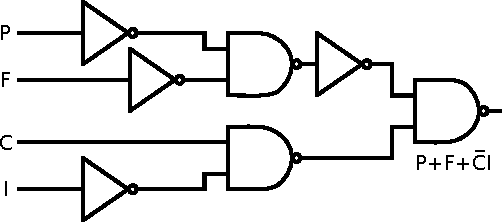
\includegraphics[width=.65\textwidth]{../E09/latex/allarme.pdf}
\caption{Circuito logico dedicato alla gestione dell'allarme in un mini-appartamento.}
\label{cir9:allarme}
\end{figure}
